\chapter{Introducción}
\label{cap:Introduccion}
El consumo de energía juega un papel muy importante en el progreso y bienestar de la sociedad. Tanto es así, que la demanda energética no deja de crecer, por ello deben llevarse a cabo medidas para reducir el consumo elevado de energía, lo que se conoce como eficiencia energética. La eficiencia energética~\cite{GarSa12} se refiere al empleo de medios de optimización en la producción y aprovechamiento de la energía, con el objetivo de proteger el medio ambiente. Esto ha pasado a ser una necesidad debido a que las emisiones de $ CO_{2} $ van en aumento y el cambio climático es un hecho.  \\

Por otro lado, puesto que las fuentes de energía fósil y nuclear son finitas, podría llegar el día en el que no se pueda satisfacer la demanda energética, salvo que se apueste por los métodos alternativos de obtención de energía. Es aquí donde entran en juego las energías renovables. Una de ellas es la energía solar~\cite{Perp12}, que permite el aprovechamiento de la radiación electromagnética del sol. Resulta interesante su estudio, debido a que es tan abundante que se considera inagotable: la cantidad de energía que el Sol vierte diariamente sobre la Tierra es diez mil veces mayor que la consumida al día en todo el planeta. Finalmente, además de ser una energía inagotable, es una energía limpia, una muy buena alternativa a los combustibles fósiles o energía nuclear. \\

Teniendo en cuenta estos dos antecedentes, existe una motivación a la hora de obtener la energía demandada de la forma mas óptima y limpia posible. Además, también debe tenerse en cuenta el factor económico. Actualmente la mayoría de particulares tienen una única fuente de suministro de energía que vendría a ser la compañía eléctrica de la cuál son clientes, importando la totalidad de la energía que su hogar demanda a dicha compañía, a un precio establecido PVPC~\cite{Ree14} (Precio voluntario al pequeño consumidor) que representa el precio máximo de referencia que pueden contratar los consumidores con hasta 10 Kwh de potencia contratada. Su valor tiene una discriminación horaria, lo que hace que en las horas de mayor consumo el precio sea mas alto. Sería interesante poder reducir la cantidad de energía que se obtiene de esta fuente en las horas pico (horas de máximo consumo donde el PVPC suele alcanzar el valor alto) y obtenerla de otra fuente cuyo precio sea menor, para así obtener un promedio mucho mas barato que con una única fuente de energía. Esto se puede lograr añadiendo nuevas fuentes al hogar, como puede ser la instalación de placas fotovoltaicas. Visto así parece muy sencillo y demasiado bueno para ser cierto, pero en el año 2015 mediante el Real Decreto 900/2015~\cite{Boe15} se establecieron unas condiciones para la instalación de placas fotovoltaicas, lo que se conoce coloquialmente como el "impuesto al sol". Por suerte, para potencias contratadas no superiores a 10 Kwh, no se pasa este impuesto, así que no es problema para el desarrollo y aplicación del sistema. Para tener el mínimo gasto posible, habría que obtener la cantidad óptima de cada una de las fuentes en cada momento, lo que supone un oficio tedioso y difícil para el ser humano. Afortunadamente para esta problemática, estamos inmersos en la era digital y las tecnologías de la información e inteligencia artificial están en auge. La inteligencia artificial~\cite{Russ06} es la ciencia encargada de construir máquinas que:
\begin{itemize}
	\item Piensan como humanos
	\item Piensan racionalmente
	\item Actúan como humanos
	\item Actúan racionalmente
\end{itemize}
Por lo tanto la inteligencia artificial podría abordar el problema definido anteriormente, mediante un sistema inteligente que se encargue de la gestión de energía automáticamente. Un sistema inteligente~\cite{Russ06} es un sistema que aprende durante su existencia como actuar para alcanzar sus objetivos, en un entorno que le rodea.\\

Con todo lo expuesto antes, se puede concluir en que este trabajo se centrará en la creación de un \textbf{sistema inteligente} para la gestión de energía en el hogar de la manera más óptima y eficiente posible. En función de un escenario determinado en una hora t (situación meteorológica, precio del kilovatio-hora (kwh) en el mercado eléctrico, nivel de carga de las baterías de almacenaje, etc) se modelará la cantidad de energía eléctrica recibida por cada una de las entradas. De igual modo, se modelará la cantidad de energía eléctrica suministrada a cada una de las salidas. Esto se traduce en una optimización y aprovechamiento de la energía, que además tiene como consecuencia un ahorro económico en la obtención de la energía necesaria.
En la Figura 1 se muestra un esquema del sistema donde se identifican desde un alto nivel de abstracción las entradas y salidas.\\

\begin{figure}[!h]
	\centering
	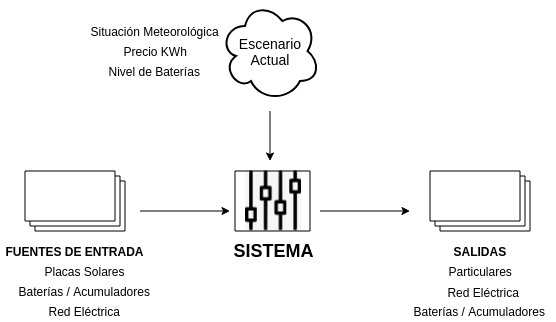
\includegraphics[width=8cm]{figs/Abstract.png}
	\caption{Dibujo del sistema}
\end{figure}

